% Options for packages loaded elsewhere
\PassOptionsToPackage{unicode}{hyperref}
\PassOptionsToPackage{hyphens}{url}
\PassOptionsToPackage{dvipsnames,svgnames,x11names}{xcolor}
%
\documentclass[
  letterpaper,
  DIV=11,
  numbers=noendperiod]{scrartcl}

\usepackage{amsmath,amssymb}
\usepackage{iftex}
\ifPDFTeX
  \usepackage[T1]{fontenc}
  \usepackage[utf8]{inputenc}
  \usepackage{textcomp} % provide euro and other symbols
\else % if luatex or xetex
  \usepackage{unicode-math}
  \defaultfontfeatures{Scale=MatchLowercase}
  \defaultfontfeatures[\rmfamily]{Ligatures=TeX,Scale=1}
\fi
\usepackage{lmodern}
\ifPDFTeX\else  
    % xetex/luatex font selection
\fi
% Use upquote if available, for straight quotes in verbatim environments
\IfFileExists{upquote.sty}{\usepackage{upquote}}{}
\IfFileExists{microtype.sty}{% use microtype if available
  \usepackage[]{microtype}
  \UseMicrotypeSet[protrusion]{basicmath} % disable protrusion for tt fonts
}{}
\makeatletter
\@ifundefined{KOMAClassName}{% if non-KOMA class
  \IfFileExists{parskip.sty}{%
    \usepackage{parskip}
  }{% else
    \setlength{\parindent}{0pt}
    \setlength{\parskip}{6pt plus 2pt minus 1pt}}
}{% if KOMA class
  \KOMAoptions{parskip=half}}
\makeatother
\usepackage{xcolor}
\setlength{\emergencystretch}{3em} % prevent overfull lines
\setcounter{secnumdepth}{-\maxdimen} % remove section numbering
% Make \paragraph and \subparagraph free-standing
\makeatletter
\ifx\paragraph\undefined\else
  \let\oldparagraph\paragraph
  \renewcommand{\paragraph}{
    \@ifstar
      \xxxParagraphStar
      \xxxParagraphNoStar
  }
  \newcommand{\xxxParagraphStar}[1]{\oldparagraph*{#1}\mbox{}}
  \newcommand{\xxxParagraphNoStar}[1]{\oldparagraph{#1}\mbox{}}
\fi
\ifx\subparagraph\undefined\else
  \let\oldsubparagraph\subparagraph
  \renewcommand{\subparagraph}{
    \@ifstar
      \xxxSubParagraphStar
      \xxxSubParagraphNoStar
  }
  \newcommand{\xxxSubParagraphStar}[1]{\oldsubparagraph*{#1}\mbox{}}
  \newcommand{\xxxSubParagraphNoStar}[1]{\oldsubparagraph{#1}\mbox{}}
\fi
\makeatother

\usepackage{color}
\usepackage{fancyvrb}
\newcommand{\VerbBar}{|}
\newcommand{\VERB}{\Verb[commandchars=\\\{\}]}
\DefineVerbatimEnvironment{Highlighting}{Verbatim}{commandchars=\\\{\}}
% Add ',fontsize=\small' for more characters per line
\usepackage{framed}
\definecolor{shadecolor}{RGB}{241,243,245}
\newenvironment{Shaded}{\begin{snugshade}}{\end{snugshade}}
\newcommand{\AlertTok}[1]{\textcolor[rgb]{0.68,0.00,0.00}{#1}}
\newcommand{\AnnotationTok}[1]{\textcolor[rgb]{0.37,0.37,0.37}{#1}}
\newcommand{\AttributeTok}[1]{\textcolor[rgb]{0.40,0.45,0.13}{#1}}
\newcommand{\BaseNTok}[1]{\textcolor[rgb]{0.68,0.00,0.00}{#1}}
\newcommand{\BuiltInTok}[1]{\textcolor[rgb]{0.00,0.23,0.31}{#1}}
\newcommand{\CharTok}[1]{\textcolor[rgb]{0.13,0.47,0.30}{#1}}
\newcommand{\CommentTok}[1]{\textcolor[rgb]{0.37,0.37,0.37}{#1}}
\newcommand{\CommentVarTok}[1]{\textcolor[rgb]{0.37,0.37,0.37}{\textit{#1}}}
\newcommand{\ConstantTok}[1]{\textcolor[rgb]{0.56,0.35,0.01}{#1}}
\newcommand{\ControlFlowTok}[1]{\textcolor[rgb]{0.00,0.23,0.31}{\textbf{#1}}}
\newcommand{\DataTypeTok}[1]{\textcolor[rgb]{0.68,0.00,0.00}{#1}}
\newcommand{\DecValTok}[1]{\textcolor[rgb]{0.68,0.00,0.00}{#1}}
\newcommand{\DocumentationTok}[1]{\textcolor[rgb]{0.37,0.37,0.37}{\textit{#1}}}
\newcommand{\ErrorTok}[1]{\textcolor[rgb]{0.68,0.00,0.00}{#1}}
\newcommand{\ExtensionTok}[1]{\textcolor[rgb]{0.00,0.23,0.31}{#1}}
\newcommand{\FloatTok}[1]{\textcolor[rgb]{0.68,0.00,0.00}{#1}}
\newcommand{\FunctionTok}[1]{\textcolor[rgb]{0.28,0.35,0.67}{#1}}
\newcommand{\ImportTok}[1]{\textcolor[rgb]{0.00,0.46,0.62}{#1}}
\newcommand{\InformationTok}[1]{\textcolor[rgb]{0.37,0.37,0.37}{#1}}
\newcommand{\KeywordTok}[1]{\textcolor[rgb]{0.00,0.23,0.31}{\textbf{#1}}}
\newcommand{\NormalTok}[1]{\textcolor[rgb]{0.00,0.23,0.31}{#1}}
\newcommand{\OperatorTok}[1]{\textcolor[rgb]{0.37,0.37,0.37}{#1}}
\newcommand{\OtherTok}[1]{\textcolor[rgb]{0.00,0.23,0.31}{#1}}
\newcommand{\PreprocessorTok}[1]{\textcolor[rgb]{0.68,0.00,0.00}{#1}}
\newcommand{\RegionMarkerTok}[1]{\textcolor[rgb]{0.00,0.23,0.31}{#1}}
\newcommand{\SpecialCharTok}[1]{\textcolor[rgb]{0.37,0.37,0.37}{#1}}
\newcommand{\SpecialStringTok}[1]{\textcolor[rgb]{0.13,0.47,0.30}{#1}}
\newcommand{\StringTok}[1]{\textcolor[rgb]{0.13,0.47,0.30}{#1}}
\newcommand{\VariableTok}[1]{\textcolor[rgb]{0.07,0.07,0.07}{#1}}
\newcommand{\VerbatimStringTok}[1]{\textcolor[rgb]{0.13,0.47,0.30}{#1}}
\newcommand{\WarningTok}[1]{\textcolor[rgb]{0.37,0.37,0.37}{\textit{#1}}}

\providecommand{\tightlist}{%
  \setlength{\itemsep}{0pt}\setlength{\parskip}{0pt}}\usepackage{longtable,booktabs,array}
\usepackage{calc} % for calculating minipage widths
% Correct order of tables after \paragraph or \subparagraph
\usepackage{etoolbox}
\makeatletter
\patchcmd\longtable{\par}{\if@noskipsec\mbox{}\fi\par}{}{}
\makeatother
% Allow footnotes in longtable head/foot
\IfFileExists{footnotehyper.sty}{\usepackage{footnotehyper}}{\usepackage{footnote}}
\makesavenoteenv{longtable}
\usepackage{graphicx}
\makeatletter
\def\maxwidth{\ifdim\Gin@nat@width>\linewidth\linewidth\else\Gin@nat@width\fi}
\def\maxheight{\ifdim\Gin@nat@height>\textheight\textheight\else\Gin@nat@height\fi}
\makeatother
% Scale images if necessary, so that they will not overflow the page
% margins by default, and it is still possible to overwrite the defaults
% using explicit options in \includegraphics[width, height, ...]{}
\setkeys{Gin}{width=\maxwidth,height=\maxheight,keepaspectratio}
% Set default figure placement to htbp
\makeatletter
\def\fps@figure{htbp}
\makeatother

\usepackage{booktabs}
\usepackage{longtable}
\usepackage{array}
\usepackage{multirow}
\usepackage{wrapfig}
\usepackage{float}
\usepackage{colortbl}
\usepackage{pdflscape}
\usepackage{tabu}
\usepackage{threeparttable}
\usepackage{threeparttablex}
\usepackage[normalem]{ulem}
\usepackage{makecell}
\usepackage{xcolor}
\KOMAoption{captions}{tableheading}
\makeatletter
\@ifpackageloaded{caption}{}{\usepackage{caption}}
\AtBeginDocument{%
\ifdefined\contentsname
  \renewcommand*\contentsname{Table of contents}
\else
  \newcommand\contentsname{Table of contents}
\fi
\ifdefined\listfigurename
  \renewcommand*\listfigurename{List of Figures}
\else
  \newcommand\listfigurename{List of Figures}
\fi
\ifdefined\listtablename
  \renewcommand*\listtablename{List of Tables}
\else
  \newcommand\listtablename{List of Tables}
\fi
\ifdefined\figurename
  \renewcommand*\figurename{Figure}
\else
  \newcommand\figurename{Figure}
\fi
\ifdefined\tablename
  \renewcommand*\tablename{Table}
\else
  \newcommand\tablename{Table}
\fi
}
\@ifpackageloaded{float}{}{\usepackage{float}}
\floatstyle{ruled}
\@ifundefined{c@chapter}{\newfloat{codelisting}{h}{lop}}{\newfloat{codelisting}{h}{lop}[chapter]}
\floatname{codelisting}{Listing}
\newcommand*\listoflistings{\listof{codelisting}{List of Listings}}
\makeatother
\makeatletter
\makeatother
\makeatletter
\@ifpackageloaded{caption}{}{\usepackage{caption}}
\@ifpackageloaded{subcaption}{}{\usepackage{subcaption}}
\makeatother

\ifLuaTeX
  \usepackage{selnolig}  % disable illegal ligatures
\fi
\usepackage{bookmark}

\IfFileExists{xurl.sty}{\usepackage{xurl}}{} % add URL line breaks if available
\urlstyle{same} % disable monospaced font for URLs
\hypersetup{
  pdftitle={Figure 1 - Maternal Mortality 2000-2017 by Country},
  pdfauthor={Mohysn Imran Malik},
  colorlinks=true,
  linkcolor={blue},
  filecolor={Maroon},
  citecolor={Blue},
  urlcolor={Blue},
  pdfcreator={LaTeX via pandoc}}


\title{Figure 1 - Maternal Mortality 2000-2017 by Country}
\author{Mohysn Imran Malik}
\date{}

\begin{document}
\maketitle


\subsection{Figure 1 - Maternal Mortality 2000-2017 by
Country}\label{figure-1---maternal-mortality-2000-2017-by-country}

Below is the script used followed by the final figure.

\begin{Shaded}
\begin{Highlighting}[]
\CommentTok{\# load packages}

\FunctionTok{library}\NormalTok{(here)}
\end{Highlighting}
\end{Shaded}

\begin{verbatim}
Warning: package 'here' was built under R version 4.4.1
\end{verbatim}

\begin{verbatim}
here() starts at C:/Users/MoMal/OneDrive/Masters/CHL8010H/Week 5/Week 5 - Table1_Figure
\end{verbatim}

\begin{Shaded}
\begin{Highlighting}[]
\FunctionTok{library}\NormalTok{(tidyverse)}
\end{Highlighting}
\end{Shaded}

\begin{verbatim}
Warning: package 'tidyverse' was built under R version 4.4.1
\end{verbatim}

\begin{verbatim}
-- Attaching core tidyverse packages ------------------------ tidyverse 2.0.0 --
v dplyr     1.1.4     v readr     2.1.5
v forcats   1.0.0     v stringr   1.5.1
v ggplot2   3.5.1     v tibble    3.2.1
v lubridate 1.9.3     v tidyr     1.3.1
v purrr     1.0.2     
\end{verbatim}

\begin{verbatim}
-- Conflicts ------------------------------------------ tidyverse_conflicts() --
x dplyr::filter() masks stats::filter()
x dplyr::lag()    masks stats::lag()
i Use the conflicted package (<http://conflicted.r-lib.org/>) to force all conflicts to become errors
\end{verbatim}

\begin{Shaded}
\begin{Highlighting}[]
\FunctionTok{library}\NormalTok{(dplyr)}
\FunctionTok{library}\NormalTok{(knitr)}
\FunctionTok{library}\NormalTok{(kableExtra)}
\end{Highlighting}
\end{Shaded}

\begin{verbatim}
Warning: package 'kableExtra' was built under R version 4.4.1
\end{verbatim}

\begin{verbatim}

Attaching package: 'kableExtra'

The following object is masked from 'package:dplyr':

    group_rows
\end{verbatim}

\begin{Shaded}
\begin{Highlighting}[]
\FunctionTok{library}\NormalTok{(here)}

\CommentTok{\# load data }

\FunctionTok{here}\NormalTok{()}
\end{Highlighting}
\end{Shaded}

\begin{verbatim}
[1] "C:/Users/MoMal/OneDrive/Masters/CHL8010H/Week 5/Week 5 - Table1_Figure"
\end{verbatim}

\begin{Shaded}
\begin{Highlighting}[]
\CommentTok{\# load dataset from project folder "original"}

\NormalTok{rawdat }\OtherTok{\textless{}{-}} \FunctionTok{read.csv}\NormalTok{(}\FunctionTok{here}\NormalTok{(}\StringTok{"original"}\NormalTok{, }\StringTok{"final\_conflict.csv"}\NormalTok{), }\AttributeTok{header =} \ConstantTok{TRUE}\NormalTok{)}
\NormalTok{rawdat }\OtherTok{\textless{}{-}} \FunctionTok{as.tibble}\NormalTok{(rawdat)}
\end{Highlighting}
\end{Shaded}

\begin{verbatim}
Warning: `as.tibble()` was deprecated in tibble 2.0.0.
i Please use `as_tibble()` instead.
i The signature and semantics have changed, see `?as_tibble`.
\end{verbatim}

\begin{Shaded}
\begin{Highlighting}[]
\FunctionTok{summary}\NormalTok{(rawdat)}
\end{Highlighting}
\end{Shaded}

\begin{verbatim}
      X.1            Year          ISO            total_droughts   
 Min.   :   1   Min.   :2000   Length:5329        Min.   :0.00000  
 1st Qu.:1333   1st Qu.:2004   Class :character   1st Qu.:0.00000  
 Median :2665   Median :2009   Mode  :character   Median :0.00000  
 Mean   :2665   Mean   :2009                      Mean   :0.06361  
 3rd Qu.:3997   3rd Qu.:2014                      3rd Qu.:0.00000  
 Max.   :5329   Max.   :2019                      Max.   :3.00000  
                                                                   
 total_earthquakes   Total_Best       bin_conflict    country_name      
 Min.   : 0.0000   Min.   :    0.0   Min.   :0.0000   Length:5329       
 1st Qu.: 0.0000   1st Qu.:    0.0   1st Qu.:0.0000   Class :character  
 Median : 0.0000   Median :    0.0   Median :0.0000   Mode  :character  
 Mean   : 0.1034   Mean   :  233.5   Mean   :0.1751                     
 3rd Qu.: 0.0000   3rd Qu.:    0.0   3rd Qu.:0.0000                     
 Max.   :11.0000   Max.   :78644.0   Max.   :1.0000                     
                                                                        
    region             gdp1000              OECD          OECD2023     
 Length:5329        Min.   :  0.1105   Min.   :0.000   Min.   :0.0000  
 Class :character   1st Qu.:  1.2383   1st Qu.:0.000   1st Qu.:0.0000  
 Mode  :character   Median :  4.0719   Median :0.000   Median :0.0000  
                    Mean   : 11.4917   Mean   :0.171   Mean   :0.1882  
                    3rd Qu.: 13.1531   3rd Qu.:0.000   3rd Qu.:0.0000  
                    Max.   :123.6787   Max.   :1.000   Max.   :1.0000  
                    NA's   :1671       NA's   :1609    NA's   :1609    
    popdens          urban             agedep          male_edu     
 Min.   : 0.00   Min.   : 0.1025   Min.   : 16.17   Min.   : 1.067  
 1st Qu.:14.79   1st Qu.:17.2872   1st Qu.: 47.94   1st Qu.: 5.904  
 Median :27.52   Median :30.2535   Median : 55.51   Median : 8.368  
 Mean   :30.57   Mean   :30.6948   Mean   : 61.94   Mean   : 8.258  
 3rd Qu.:40.72   3rd Qu.:41.6558   3rd Qu.: 77.11   3rd Qu.:10.849  
 Max.   :99.86   Max.   :93.4135   Max.   :111.48   Max.   :14.441  
 NA's   :1629    NA's   :1629      NA's   :1609     NA's   :1629    
      temp         rainfall1000          X        Maternal.Mortality
 Min.   :-2.405   Min.   :0.0199   Min.   :   1   Min.   :   2.0    
 1st Qu.:12.928   1st Qu.:0.5915   1st Qu.:1331   1st Qu.:  20.0    
 Median :21.958   Median :1.0129   Median :2660   Median :  78.0    
 Mean   :19.625   Mean   :1.2022   Mean   :2660   Mean   : 220.5    
 3rd Qu.:25.869   3rd Qu.:1.6871   3rd Qu.:3990   3rd Qu.: 331.8    
 Max.   :29.676   Max.   :4.7108   Max.   :5320   Max.   :2480.0    
 NA's   :1629     NA's   :1629     NA's   :9      NA's   :1135      
 Infant.Mortality  Neonatal.Mortality Under.5.Mortality
 Min.   :  1.600   Min.   : 0.80      Min.   :  1.800  
 1st Qu.:  8.409   1st Qu.: 5.30      1st Qu.:  9.992  
 Median : 21.100   Median :13.18      Median : 24.900  
 Mean   : 29.836   Mean   :16.83      Mean   : 41.851  
 3rd Qu.: 46.400   3rd Qu.:26.45      3rd Qu.: 64.600  
 Max.   :138.100   Max.   :60.90      Max.   :224.900  
 NA's   :509       NA's   :509        NA's   :509      
\end{verbatim}

\begin{Shaded}
\begin{Highlighting}[]
\CommentTok{\# select only needed variables (Country name, ISO, Year, Maternal mortality) and select for only years \textless{}2018}
\NormalTok{df\_trend }\OtherTok{\textless{}{-}}\NormalTok{ rawdat }\SpecialCharTok{\%\textgreater{}\%} \FunctionTok{select}\NormalTok{(country\_name, ISO, Year, Maternal.Mortality) }\SpecialCharTok{\%\textgreater{}\%} 
  \FunctionTok{filter}\NormalTok{(Year }\SpecialCharTok{\textless{}} \DecValTok{2018}\NormalTok{)}

\CommentTok{\#isolate only countries in which there was an increase in maternal mortality between 2000 and 2017 and create a vector of their names}
\NormalTok{up\_trend }\OtherTok{\textless{}{-}}\NormalTok{ df\_trend }\SpecialCharTok{\%\textgreater{}\%} 
  \FunctionTok{filter}\NormalTok{(Year }\SpecialCharTok{==} \DecValTok{2000} \SpecialCharTok{|}\NormalTok{ Year }\SpecialCharTok{==} \DecValTok{2017}\NormalTok{) }\SpecialCharTok{\%\textgreater{}\%} 
  \FunctionTok{arrange}\NormalTok{(ISO, Year) }\SpecialCharTok{\%\textgreater{}\%} 
  \FunctionTok{group\_by}\NormalTok{(ISO) }\SpecialCharTok{\%\textgreater{}\%} 
  \FunctionTok{mutate}\NormalTok{(}\AttributeTok{diffmatmor =}\NormalTok{ Maternal.Mortality }\SpecialCharTok{{-}}\NormalTok{ Maternal.Mortality[}\DecValTok{1}\NormalTok{L]) }\SpecialCharTok{\%\textgreater{}\%} 
  \FunctionTok{filter}\NormalTok{(diffmatmor }\SpecialCharTok{\textgreater{}} \DecValTok{0}\NormalTok{)}

\CommentTok{\#Remove rows with missing data}
\NormalTok{up\_trend }\OtherTok{\textless{}{-}}\NormalTok{ up\_trend[}\DecValTok{1}\SpecialCharTok{:}\DecValTok{13}\NormalTok{,]}

\CommentTok{\#make a vector with all of our countries to include in the figure and then subset our df\_trend dataset for these countries}
\NormalTok{countries\_trend }\OtherTok{\textless{}{-}} \FunctionTok{c}\NormalTok{(}\StringTok{"Brunei"}\NormalTok{, }\StringTok{"Canada"}\NormalTok{, }\StringTok{"Dominican Republic"}\NormalTok{, }\StringTok{"Haiti"}\NormalTok{, }
                    \StringTok{"Jamaica"}\NormalTok{, }\StringTok{"Kuwait"}            
\NormalTok{                    , }\StringTok{"Lebanon"}\NormalTok{, }\StringTok{"Libya"}\NormalTok{,             }
                    \StringTok{"Saint Lucia"}\NormalTok{,}\StringTok{"Mauritius"}         
\NormalTok{                    ,}\StringTok{"Syria"}\NormalTok{, }\StringTok{"United States"}     
\NormalTok{                      ,}\StringTok{"Venezuela"}\NormalTok{)}
\NormalTok{final\_trend }\OtherTok{\textless{}{-}}\NormalTok{ df\_trend }\SpecialCharTok{\%\textgreater{}\%} \FunctionTok{filter}\NormalTok{(country\_name }\SpecialCharTok{\%in\%}\NormalTok{ countries\_trend)}

\CommentTok{\#Plot trend using ggplot}
\FunctionTok{ggplot}\NormalTok{(final\_trend, }\FunctionTok{aes}\NormalTok{(}\AttributeTok{x =}\NormalTok{ Year, }\AttributeTok{y =}\NormalTok{ Maternal.Mortality, }\AttributeTok{color =}\NormalTok{ country\_name)) }\SpecialCharTok{+}
  \FunctionTok{geom\_line}\NormalTok{(}\AttributeTok{size =} \DecValTok{1}\NormalTok{) }\SpecialCharTok{+}        
  \FunctionTok{geom\_point}\NormalTok{() }\SpecialCharTok{+}               
  \FunctionTok{labs}\NormalTok{(}
    \AttributeTok{title =} \StringTok{"Maternal Mortality Trends (2000{-}2017)"}\NormalTok{,}
    \AttributeTok{x =} \StringTok{"Year"}\NormalTok{,}
    \AttributeTok{y =} \StringTok{"Maternal Mortality Rate"}\NormalTok{,}
    \AttributeTok{color =} \StringTok{"Country"}
\NormalTok{  ) }\SpecialCharTok{+}
  \FunctionTok{theme\_minimal}\NormalTok{() }\SpecialCharTok{+}           
  \FunctionTok{scale\_color\_hue}\NormalTok{()}
\end{Highlighting}
\end{Shaded}

\begin{verbatim}
Warning: Using `size` aesthetic for lines was deprecated in ggplot2 3.4.0.
i Please use `linewidth` instead.
\end{verbatim}

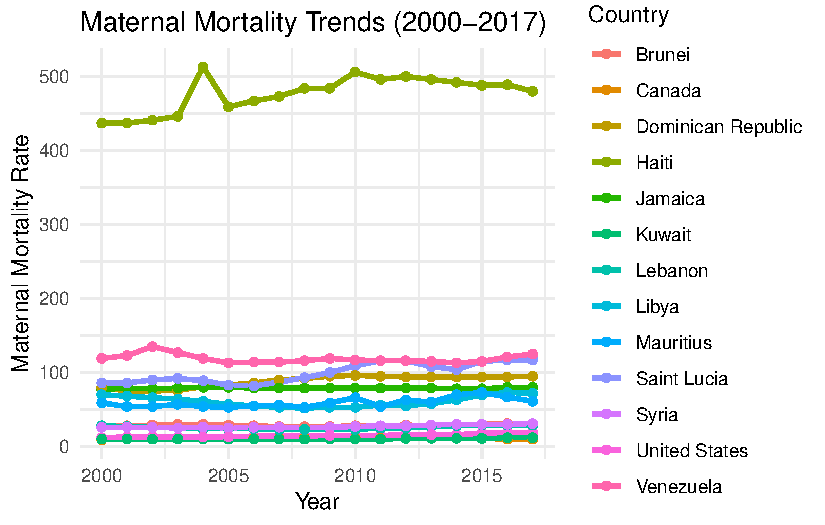
\includegraphics{figure1_files/figure-pdf/unnamed-chunk-1-1.pdf}




\end{document}
